\section{Experimental Setup}
We evaluate prediction under controlled characterization budgets, then measure how estimates affect native extraction and timing. Each evaluation fixes the support and reference appropriate to its task.

\subsection{Data and Training}
Table~\ref{tab:data} distinguishes public process rules from FEM cross sections. Of 1,713 public rows, the original split has 1,116/256/341 train/validation/test rows. Reserving native tables removes 55 training and nine validation rows. Deduplication removes another 10/1/1 rows from the three reported views, accounting for the difference of 76. The retrospective confirmation view retains 20 of the 84 native holdouts. The native and retrospective evaluations therefore share these test tables. The transfer setting fits and selects models on FreePDK15 and supplies only observed ASAP7 labels at evaluation.
\begin{table}[t]\centering
\caption{Source opportunities and evaluation populations. Counts in the first row are deduplicated fitting, selection and confirmation tables. Updates are per member. A dash indicates an unavailable control.}\label{tab:data}
\small\begin{tabular}{@{}lrrr@{}}\toprule
 & Public & FEM & Transfer\\\midrule
Tables & 1051/246/340 & 16/24/16 & 8/12/8\\
Budget-eligible tables & 338 & 16 & 8\\
Fit/confirm nodes per table & varies & 153/128 & 153/128\\
Fusion updates ($10^3$) & 24 & 12 & 12\\
MLP/CNP/AC updates ($10^3$) & 3/3/-- & 3/3/3 & 3/3/3\\\bottomrule
\end{tabular}
\end{table}
The three matched variants start from residual initializers trained for 2,000 source updates. AdamW uses learning rate $2\times10^{-4}$ and weight decay $10^{-4}$. Each reported ensemble averages three trained members. Public rules supply two per-length capacitances in source-rule units. FEM supplies three projected components in F/m. The six independent template contexts use all 153 characterization samples per context.

\subsection{Evaluation Protocols and Baselines}
For each requested holdout (10, 30, 50 or 70\%), we withhold the nearest integer number of nodes, retaining at least one support and one query. Random masks sample without replacement, block masks select a contiguous interval in coordinate order, and boundary masks remove the upper end. Training also includes eligible whole-width masks. Methods share feasible support/query episodes and mask seeds 11/29/47/71/101. Random and block queries are scored inside and outside support, boundary queries outside. Rounded masks can coincide on small tables.

Fixed-budget evaluation uses sealed queries and common geometry-selected support, with seeds 11/29/47. Public budgets are $B=4,8$, with $B=16,32,64$ also feasible for FEM and transfer. OpenRCX and MLI-ext.\ are the primary kernels. Anchor, validation-selected GP, local affine interpolation, PCHIP and inverse-distance weighting (IDW) control for the numerical basis. CNP conditions on the support directly. The MLP and component-supervised adapted AttentionCap (AC) receive 200 and 50 target-fitting steps, respectively. Source validation compares two learning rates and three adaptation lengths for each. CNP uses two candidate learning rates and receives no target updates. AC retains its Transformer and symmetric output head~\cite{attentioncode}. Shared observations control the budget even though fitting opportunities differ.

Native evaluation fixes routed AES and IBEX layouts, libraries and constraints on ASAP7, GF180, IHP SG13G2 and Sky130HS (OpenROAD \texttt{0b54bb3203}). Fixed-node export completes 83 eligible held-out tables at $B=4,8$ using common farthest-point supports capped by candidate availability. A two-node ASAP7 OVER table retains its original observations. Full-support compute-table population uses the original characterization and an eligible-slot hook. Each protocol compares against extraction with the original full rules on the same layout.

\subsection{Runtime Measurement}
Direct predictors and resident FEM use one pinned Xeon Gold 6530 thread. Three warmups precede 20 interleaved predictor timing blocks. Batch limits of 1, 8 and 32 queries have separate accuracy measurements. Warm costs include encoding, applicable corrections, ensemble inference and output assembly. Single-request latency measures one query, whereas amortized cost divides batch wall time by the actual number of queries. One-time target fitting includes first-use optimizer initialization. Target fitting, source training, export, native extraction, SPEF output and STA are recorded separately. The compute-table inventory requires a first extraction because OpenRCX defers rule loading.

\begin{figure*}[t]\centering
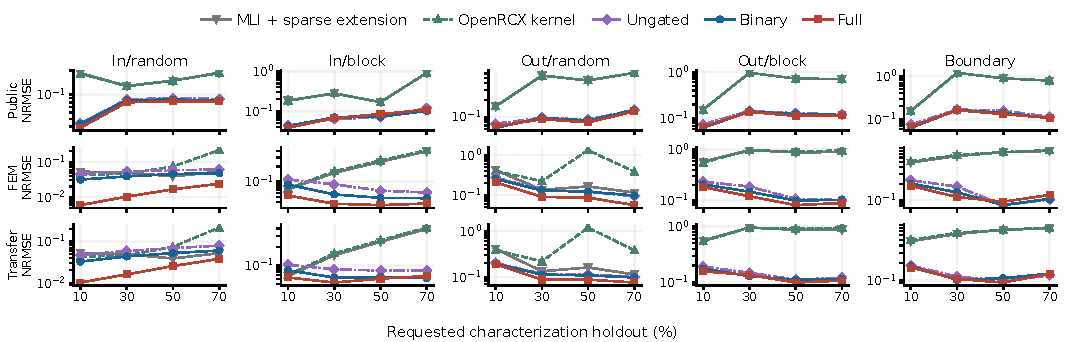
\includegraphics[width=\textwidth]{figures/coverage_four_ratios.pdf}
\caption{Macro NRMSE at four requested holdout levels. Each domain includes inside/outside random and block queries and outside boundary queries. Each point averages mask-level scores on the same feasible episodes.}\label{fig:coverage}
\end{figure*}

\subsection{Metrics}
For a component group $g$ with query indices $Q_g$, the normalized root-mean-square error is
\begin{equation}
E_g=\sqrt{\sum_{i\in Q_g}(\widehat y_i-y_i)^2\big/\sum_{i\in Q_g}y_i^2}.
\end{equation}
Coverage results average $E_g$ over nonzero-energy groups defined by process, family and component, and then over masks. Fixed-budget scores pool the three data seeds before group normalization. The independent physical comparison averages errors by family and component, whereas support-continuation scores average member-wise group-balanced errors. For native extraction we compare matched-net capacitances and absolute deviations in worst slack (WS), total negative slack (TNS) and matched endpoint slack against full-rule extraction.
\section{Results}
We first ask how the estimators respond to characterization coverage and fixed budgets. An independent template reference tests whether corrections help when the entire support is available. Native extraction then tests whether prediction gains carry through to nets and timing endpoints, and identifies where deployment incurs cost.

\subsection{Characterization Coverage Sensitivity}

Figure~\ref{fig:coverage} comprises 60 domain--coverage--holdout conditions. Full achieves lower error than both kernels in 60, Binary in 55 and Ungated in 50. Full improves on Binary in 49 and on Ungated in 55. Equal weighting of condition scores gives mean NRMSE of 0.0879 for Full, 0.4806 for OpenRCX and 0.4204 for MLI-ext., reductions of 81.7\% and 79.1\% relative to the corresponding means. Complete MLI cells cover 35,362 of 171,315 requested query instances (20.64\%). The remaining requests use boundary or sparse-support handling.

At 10, 30, 50 and 70\% holdout, Full has mean errors of 0.1000, 0.0874, 0.0780 and 0.0861, respectively. The domain means are 0.0927 on public rules, 0.0822 on FEM and 0.0887 on transfer. Mean error increases from 0.0475 inside support to 0.1148 outside. The populations and reference energies vary with the mask. The 60 conditions share tables and queries. On public inside/block queries at 50\% holdout, Ungated and Binary achieve 0.0704 and 0.0731 against Full's 0.0849. On FEM inside/block queries at 10\%, Full achieves 0.0534 against 0.1104 and 0.0874. Full's narrowest margin over the lower-error kernel is 5.25\% (transfer, inside/block, 10\%). Its paired interval includes zero with just two layer groups. The repeated improvement across evaluated conditions motivates Full as the default, while individual simplified variants retain local advantages.

\subsection{Fixed-Budget Learning Comparisons}
\begin{figure}[t]\centering
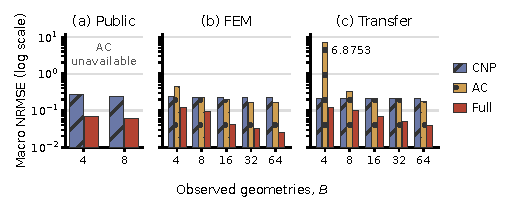
\includegraphics[width=\columnwidth]{figures/fixed_budget_controls.pdf}
\caption{Fixed-budget macro NRMSE on common observations and sealed queries (log scale). AC is component-supervised adapted AttentionCap. Public AC results are unavailable.}\label{fig:budget_controls}
\end{figure}
Full has lower error than CNP in all 12 available domain--budget settings and adapted AC in all ten FEM/transfer settings (Fig.~\ref{fig:budget_controls}). On public rules at $B=4/8$, its errors are 0.0708/0.0609 against CNP's 0.2650/0.2374. On FEM, increasing $B$ from 4 to 64 reduces Full's error from 0.1233 to 0.0250 and AC's from 0.4546 to 0.1657. These comparisons concern the component-supervised adaptation and its specific fitting budget. At FEM $B=4$ the target-fitted MLP is more accurate (0.0515).

\subsection{Physical Reference and Cross-Process Transfer}
Transfer uses held-out ASAP7 table values. From $B=4$ to 64, Full improves from 0.1182 to 0.0386, compared with 6.8753 to 0.1791 for AC. At $B=64$, MLP and GP achieve lower errors of 0.0264 and 0.0271. Ungated obtains 0.0814 on transfer and 0.0609 on FEM at that budget. Target fitting, numerical smoothness and learned corrections thus have different operating ranges.

The independent test uses 71 layout-parameterized, off-node geometries in six ASAP7 M4/M5 contexts. Logged widths and spacings define symmetric equal-width side conductors, finite grounded planes and a grounded exterior boundary. P2 FEM solves supply Maxwell matrices from which ground and summed lateral capacitance are projected. With all 153 samples per context, direct Anchor, Full and Binary errors are 0.00451, 0.01675 and 0.02218. On these templates, the available samples already support accurate numerical interpolation. The reference describes the specified cross sections and boundary conditions.

\subsection{Native Extraction and Timing Fidelity}
\begin{table}[t]\centering
\caption{Fixed-node export (left) and full-support compute-table deployment (right). Both use the same eight layouts and their original full-rule extractions as reference.}\label{tab:deployment}
\begingroup
\fontsize{5.8}{6.5}\selectfont
\setlength{\tabcolsep}{0.75pt}\setlength{\arrayrulewidth}{0.25pt}
\renewcommand{\arraystretch}{1.0}
\newcommand{\layoutspan}[1]{\raisebox{-3.25pt}[0pt][0pt]{#1}}
\begin{tabular*}{\columnwidth}{@{\extracolsep{\fill}}|l|c||rrr|rrr||rrrrr|}
\hline
\multicolumn{2}{|c||}{\textbf{Layout / budget}} & \multicolumn{6}{c||}{\textbf{Rule-export: error reduction (\%)}} & \multicolumn{5}{c|}{\textbf{Full-support compute table}} \\
\cline{3-13}
 & & \multicolumn{3}{c|}{vs. MLI-ext.} & \multicolumn{3}{c||}{vs. OpenRCX} & \multicolumn{5}{c|}{Fidelity and preparation / extraction cost} \\
\cline{3-13}
\textbf{Layout} & $B$ & C & WS & TNS & C & WS & TNS & C err. & Prep. & PEX & SPEF & $T/T_0$ \\
\hline
\layoutspan{\textbf{ASAP7/AES}} & 4 & 81.2 & 89.7 & 84.1 & 81.1 & 89.6 & 84.0 & \layoutspan{0.00426} & \layoutspan{5.41} & \layoutspan{2.05} & \layoutspan{0.49} & \layoutspan{0.991} \\
 & 8 & 89.1 & 88.4 & 89.5 & 89.0 & 88.4 & 89.5 &  &  &  &  &  \\
\hline
\layoutspan{\textbf{ASAP7/IBEX}} & 4 & 81.4 & 90.3 & 85.6 & 81.3 & 90.2 & 85.5 & \layoutspan{0.00516} & \layoutspan{5.41} & \layoutspan{3.30} & \layoutspan{0.72} & \layoutspan{1.020} \\
 & 8 & 89.2 & 98.3 & 96.7 & 89.2 & 98.3 & 96.7 &  &  &  &  &  \\
\hline
\layoutspan{\textbf{GF180/AES}} & 4 & 84.6 & 85.0 & 84.4 & 84.6 & 85.0 & 84.4 & \layoutspan{0.00030} & \layoutspan{8.39} & \layoutspan{2.45} & \layoutspan{0.52} & \layoutspan{1.031} \\
 & 8 & 78.7 & 78.5 & 78.3 & 78.7 & 78.5 & 78.3 &  &  &  &  &  \\
\hline
\layoutspan{\textbf{GF180/IBEX}} & 4 & 84.5 & 85.1 & 84.4 & 84.5 & 85.1 & 84.4 & \layoutspan{0.00020} & \layoutspan{8.39} & \layoutspan{2.73} & \layoutspan{0.52} & \layoutspan{0.999} \\
 & 8 & 78.4 & 78.7 & 77.7 & 78.4 & 78.7 & 77.7 &  &  &  &  &  \\
\hline
\layoutspan{\textbf{IHP/AES}} & 4 & 91.3 & 94.5 & -- & 91.3 & 94.5 & -- & \layoutspan{0.05656} & \layoutspan{13.99} & \layoutspan{2.00} & \layoutspan{0.40} & \layoutspan{1.035} \\
 & 8 & 87.4 & 90.1 & -- & 87.4 & 90.1 & -- &  &  &  &  &  \\
\hline
\layoutspan{\textbf{IHP/IBEX}} & 4 & 92.5 & 93.3 & 100.0 & 92.5 & 93.3 & 100.0 & \layoutspan{0.05477} & \layoutspan{13.99} & \layoutspan{3.10} & \layoutspan{0.66} & \layoutspan{1.029} \\
 & 8 & 87.6 & 88.2 & -- & 87.5 & 88.1 & -- &  &  &  &  &  \\
\hline
\layoutspan{\textbf{Sky130/AES}} & 4 & 89.7 & 94.5 & 97.1 & 89.9 & 94.6 & 97.1 & \layoutspan{0.00382} & \layoutspan{8.48} & \layoutspan{2.43} & \layoutspan{0.56} & \layoutspan{1.017} \\
 & 8 & 87.3 & 83.5 & 76.6 & 87.3 & 83.1 & 76.2 &  &  &  &  &  \\
\hline
\layoutspan{\textbf{Sky130/IBEX}} & 4 & 88.4 & 91.1 & 89.6 & 88.6 & 91.2 & 89.8 & \layoutspan{0.00233} & \layoutspan{8.48} & \layoutspan{2.29} & \layoutspan{0.58} & \layoutspan{1.024} \\
 & 8 & 85.6 & 78.0 & 81.7 & 85.6 & 77.4 & 81.1 &  &  &  &  &  \\
\hline
\end{tabular*}
\par\vspace{2pt}
\parbox{\columnwidth}{\fontsize{6}{6.7}\selectfont Rule-export values average seeds 11/29/47. C denotes capacitance NRMSE. WS/TNS are absolute timing deviations from full-table extraction. ``-- means both errors are zero. Compute table: C err. is net-C NRMSE. Prep./PEX/SPEF are in seconds. $T/T_0$ is the mean extraction ratio over three release runs. Preparation includes inventory and loading. Native table construction/injection stays within PEX. Shared right-hand values use full characterization, not the row budget $B$.}
\endgroup

\end{table}
At both rule-export budgets, Full reduces net-capacitance NRMSE and absolute WS deviation relative to each kernel on every layout (Table~\ref{tab:deployment}). TNS deviation decreases in 13 of the 16 cells and is zero for both methods in three. For GF180/IBEX at $B=8$, MLI-ext.\ and Full yield net-capacitance NRMSE of 0.0161 and 0.00348, WS deviations of 38.25 and 8.14\,ps, and TNS deviations of 52.74 and 11.77\,ns. Comparing Full directly with Binary gives six net-capacitance wins and four WS wins. Binary has smaller P99 endpoint error in ten cells.
\begin{figure}[t]\centering
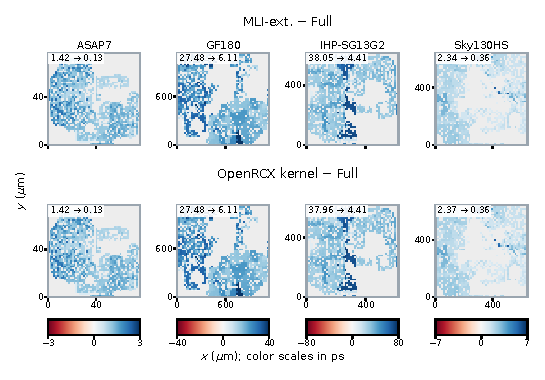
\includegraphics[width=\columnwidth]{figures/downstream_two_kernels.pdf}
\caption{Reduction in absolute endpoint slack error (ps) at $B=8$, relative to MLI-ext.\ (top) and OpenRCX (bottom). Columns show ASAP7, GF180, IHP and Sky130HS IBEX. Each $50\times50$ map averages gains over endpoints and three seeds. Blue indicates improvement, red degradation and gray empty bins.}\label{fig:spatial}
\end{figure}
For endpoint $j$ and seed $r$, we measure $|s_{jr}-s_j^{\rm original}|$ in ps. We join finite slacks by endpoint name and average over endpoints and seeds to obtain mean absolute error (MAE) for each method. We report one minus the ratio of Full's MAE to the baseline MAE. The P99 summary instead takes the 99th percentile of absolute error within each run before averaging seeds. Figure~\ref{fig:spatial} contains 3,704/2,039/3,704/3,975 endpoints per seed on the four IBEX layouts. Relative MAE reductions span 77.8--91.1\% against the two kernels, with lower MAE in all 12 layout--seed pairs for each kernel.

In the full-support internal protocol, pass-through preserves logged returns and electrical SPEF records on all eight layouts. Preparation covers 49,657 finite slots across four libraries and changes 924,647 traced getter returns. Full's net-capacitance NRMSE ranges from 0.00020 to 0.05656. IHP exhibits the largest WS deviations, 74.4\,ps on AES and 147.4\,ps on IBEX. These deviations measure agreement with the native full rules. In a separate paired sparse-native test, Full improves net-capacitance, WS and P99 over Native-sparse in 7, 9 and 7 of 16 cells, respectively. Full improves all three metrics over Binary-native in all 16. At fixed-node $B=4$, equal-layout mean P99 is 4.25\,ps for Full and 2.01\,ps for Binary. At the sparse-native interface, Full also has lower endpoint MAE than Native-sparse in eight cells. The distinction between preparing internal slots and exporting fixed nodes therefore affects downstream comparisons.

\subsection{Preparation and Runtime Cost}
On the 71 physical queries, warm Full, Binary and Anchor cost 3.706, 2.110 and 0.788\,ms/query at the amortized setting. Full averages 40.97\,ms for a single request. Target fitting across six contexts costs 14.03\,s for the MLP and 11.27\,s for AC. These timings distinguish direct prediction from preparing a library for multiple designs.

At $B=8$ and seed 11, prediction, payload writing and fixed-node export for four libraries cost 0.70/0.67/0.91\,s for MLI-ext./Binary/Full after 0.88\,s of shared loading and support selection. The MLI-ext.\ timing uses the output-equivalent CMI implementation. In 96 release runs, Full's mean extraction/original ratio ranges from 0.983 to 1.047 across layouts. In 120 separate full-support compute-table runs, Full's corresponding ratio is 0.991--1.035. Charging inventory, external preparation and process residual gives first-design PEX overhead of 161.1--670.4\% from measured stage sums. Table construction and injection fall inside PEX. Reuse amortizes preparation across designs while layout queries retain native evaluation.
\ifdefined\CapFillExtended% Supporting figures and tables share the reference populations of the six-section text.
\onecolumn
\small
\makeatletter
\newcommand{\detailtable}[3]{\par\medskip\noindent\begin{minipage}{\linewidth}
\centering\def\@captype{table}\caption{#2}\label{xt:#1}\small\setlength{\tabcolsep}{4pt}\input{detail/#3.tex}\end{minipage}\par\medskip}
\newcommand{\detailfigure}[3]{\par\medskip\noindent\begin{minipage}{\linewidth}
\centering\includegraphics[width=#2\linewidth,height=.32\textheight,keepaspectratio]{detail/#1}\def\@captype{figure}\caption{#3}\label{xf:#1}\end{minipage}\par\medskip}
\makeatother
\subsection{Coverage by Domain and Support Region}
Tables~\ref{xt:public}--\ref{xt:transfer} give the absolute scores behind the coverage comparisons. Each entry describes an ensemble prediction or a deterministic kernel on common feasible queries. The selected GP uses source validation. Adjacent percentages may produce identical withheld sets on short curves. Of 21,840 feasible support/query episodes, 11,245 repeat a rounded support/query identity. The five masks within each independent table group remain together in paired uncertainty calculations.

\detailtable{public}{Public-rule coverage. ORCX denotes the pinned OpenRCX kernel. Errors are mean-mask macro NRMSE.}{coverage_public}
\detailtable{fem}{FEM confirmation coverage under the same estimator and aggregation.}{coverage_reference}
\clearpage
\detailtable{transfer}{FreePDK15-to-ASAP7 transfer. Only the available target support carries target labels during inference.}{coverage_to_asap7}
\detailtable{numerical}{All numerical component controls at 30\% holdout on the same evaluation cells. Lower macro NRMSE is better.}{numerical_30percent}
Table~\ref{xt:numerical} separates applicability from typical accuracy. At 30\% holdout, local affine extrapolation gives 0.0389 in the FEM inside/random cell, and Full gives 0.0103. In other cells the ordering reverses. The worst ratios to the lower-error kernel across all 60 conditions are 0.948 for Full, 1.349 for Binary, and 1.778 for Ungated. The narrowest Full margin arises on eight transfer tables grouped into two target layers. The paired interval for Full minus the lower-error kernel is $[-0.01098,0.00534]$ in that cell. The five masks share the same two layer groups. Across all cells, Binary beats OpenRCX in 58 and MLI-ext.\ in 55, and Ungated beats them in 54 and 52. A source-fitted fixed mixture of frozen candidates improves on both kernels in 51 conditions. Separately trained numerical-only and no-agreement gates achieve 29 and 59 strict wins, respectively. The numerical-only control removes both the Transformer state and the neural candidates. It therefore tests their combined contribution.
\clearpage
\subsection{Fixed Budgets and Support-Protocol Controls}
\detailfigure{budget_accuracy}{.90}{Pooled-replicate macro NRMSE on sealed queries for three data seeds. The MLP adapts on the observed target support. Full and Binary reuse source-trained parameters. Only feasible budgets are shown.}
\detailtable{aux}{Additional fixed-budget controls. AC denotes component-supervised adapted AttentionCap. A dash marks an unavailable or infeasible comparison.}{budget_aux}
\detailfigure{support_protocol}{.66}{Mean-member, group-balanced error after matched continuation. H uses the original support distribution and L buys a fixed number of observations selected for coverage.}
Figure~\ref{xf:budget_accuracy} and Table~\ref{xt:aux} compare predictors at fixed budgets. In Fig.~\ref{xf:support_protocol}, the three source seeds receive 2,000 matched continuation steps per member. Binary-L gives lower error on average at $B=4,8$. Full-L is more accurate than Binary-L at $B=16,32$ but loses 20.0\% and 28.9\% relative to the source-trained Full at these budgets. In a separate reverse-direction MLP evaluation from ASAP7 to FreePDK15, target fitting reduces NRMSE from 0.4414 without updates to 0.0569 at $B=4$ and 0.0284 at $B=64$. Low-budget continuation changes both observation count and spatial coverage. Across 1,728 dependent component/seed/cell outcomes, Full-L has lower, equal or higher capacitance P99 than Binary-L in 887, 225 and 616 cases. These are table-component tails. The native STA assessment instead uses endpoint slack tails.
\clearpage
\subsection{Native Fidelity Under Fixed-Node Export}
\detailfigure{native_fidelity}{.93}{Fixed-node export on each layout. Top panels use 30/50\% block holdouts. Net-capacitance NRMSE averages seeds and WS/TNS deviations take the maximum absolute value. Bottom panels average three seed-level scores at $B=4,8$. P99 is computed over absolute endpoint slack errors within a run.}
\detailtable{export}{Three-seed means on each layout and budget. C is net-capacitance NRMSE. WS and P99 are absolute slack errors in ps. MLI uses the declared extension.}{rule_export_absolute}
Figure~\ref{xf:native_fidelity} distinguishes block holdout from fixed budgets. In Table~\ref{xt:export}, at GF180/IBEX and $B=4$, Full's P99 exceeds Binary's by 7.64\,ps. At $B=4$, equal-layout mean P99 errors are 4.25 and 2.01\,ps, respectively. Full improves, ties or worsens TNS deviation relative to Binary in 5/4/7 conditions. Full and Binary have identical false-negative counts in all 16 cells, while false-positive counts tie in 14 and increase for Full in two. Under 50\% block holdout on GF180/IBEX, Full reduces maximum WS deviation from 132.8 to 37.01\,ps and maximum TNS deviation from 168.6 to 50.22\,ns relative to multilinear completion. These maxima give a different summary from the seed means at fixed budgets.
\clearpage
\subsection{Reference Physics and Native Agreement}
\detailfigure{query_errors}{.92}{Occurrence and error by nearest-support distance. Occurrence uses inverse inclusion probabilities. All methods share the same distance bins and the same symmetric template reference.}
\detailtable{physical}{Complete physical-template support. NRMSE is family/component balanced. P95 is the nonzero-component absolute error in pF/m. Compute-table evaluations include native geometry mapping.}{production_kernels}
\detailtable{replay}{Reference-specific errors. Native agreement uses 480 queries. FEM unique evaluates 71 templates, and FEM weighted accounts for sampling probability. Time is warm ms/query on the FEM set.}{offgrid_runtime}
For Fig.~\ref{xf:query_errors} and Tables~\ref{xt:physical}--\ref{xt:replay}, geometry-only stratification fixed 12 pilot and 71 formal queries before solving. All pass coarse/fine and doubled-domain checks, and 12 on-grid controls reproduce the saved matrices. The formal widths are 0.024 and 0.032\,$\mu$m. The macro normalized reference uncertainty is 0.00016. With the same template samples, ideal continuous distance yields OpenRCX kernel error 0.00635 against 0.01072 with native mapping and quantization. Full evaluated through populated tables gives 0.02447 compared with 0.01675 at direct query coordinates. This comparison changes batching and native mapping together.

The validated native getter counterpart takes 1.72\,ns/query in warm C++ loops after context and width resolution, versus 0.567\,$\mu$s/query through a ctypes loop. Both measure a numerical service with a resolved context. Native calibration materials and the physical template do not define identical reference problems.
\clearpage
\subsection{Warm Evaluation, Fitting and Source Cost}
\detailfigure{runtime_accuracy}{.90}{Accuracy and cost. Batch limits of 32, 8 and 1 use circles, squares and triangles. The solver marker compares against the certified fine reference. Native timing ratios and four-library export costs have their own fixed-node protocol.}
\detailtable{runtime}{Warm single-thread predictor measurements on 71 FEM templates. Amortized time, mean single-request latency and its P95 are in ms. Fit denotes the one-time cost over six contexts in seconds.}{runtime_detail}
\detailtable{source}{Measured final training-stage wall seconds summed over three members. Rows differ in hardware and source opportunity. A dash denotes an unavailable receipt. Characterization, initialization and selection add further cost.}{source_training_costs}
Figure~\ref{xf:runtime_accuracy} separates direct evaluation, extraction and preparation. Tables~\ref{xt:runtime} and~\ref{xt:source} report warm service and source training. After a reusable fit, MLP costs 0.025\,ms/query and adapted AC costs 0.230\,ms/query. Full's single-request latency includes the geometry and material sequence for that request. Increasing batch size changes its query-to-query attention as well as its throughput. A resident one-right-hand-side P2 solve takes 3.719\,s/query including meshing, assembly and factorization. Cold fine-only solves and three-level certification over the 71 geometries take 316.1 and 799.1\,s. The supplied 918 support geometries carry 4,889.83\,s of recorded fine-solver CPU work (11,761.63\,s with certification). These inputs are reused across evaluations.
\clearpage
\detailfigure{runtime_native_agreement}{.59}{Native-agreement timing over 480 queries for batch limits of 1, 8 and 32. The compiled getter counterpart supplies a reference for arithmetic and lookup after width resolution.}
{\renewcommand{\arraystretch}{0.86}\detailtable{stages}{Full-support internal deployment. PEX, its sample SD, SPEF, STA and external preparation are seconds. Each layout/mode has three release repeats. C err.\ is net-capacitance NRMSE against original rules. $\Delta$slack is in ps.}{native_stages}}
Figure~\ref{xf:runtime_native_agreement} measures direct evaluation. In Table~\ref{xt:stages}, the internal API loads rules during extraction. Its first inventory extraction is charged to preparation. The four-library rule-export comparison instead charges a single shared load of data, model bundle and supports. A complete model bundle can serve both designs in each process. The reported first-design estimates sum measured stages including process residual. External Python startup and imports were outside the preparation timers.
\clearpage
\subsection{Matched Sparse-Native Interface}
Fixed-node export and full-support slot replacement use different support and runtime contracts. A third experiment physically removes hidden characterization rows before constructing the sparse native rule. Each of four arms uses the same support, native getter and original full-rule layout reference on eight layouts, two budgets and three support seeds. This gives 48 paired settings and 192 arm-settings. Hidden-label replacement tests on ASAP7 and IHP reproduce the Binary and Full predictions bit for bit.

\detailtable{sparse}{Three-seed means with the same sparse-native interface. C is net-capacitance NRMSE, WS absolute worst-slack deviation in ps. Native denotes Native-sparse. MLI denotes MLI-ext.-native.}{native_sparse_accuracy}
\detailtable{tails}{Sparse-native timing tails. P99 denotes absolute endpoint slack error in ps, TNS absolute deviation in ns.}{native_sparse_tails}
Across Tables~\ref{xt:sparse} and~\ref{xt:tails}, Full improves all three reported net-C/WS/P99 metrics over Binary-native in all 16 cells. Compared with Native-sparse, its win counts are 7/16, 9/16 and 7/16, respectively. IHP contributes large absolute deviations. These observations bound the extent to which offline coverage consistency transfers to a new deployment interface.
\normalsize
\fi
